%!TEX root = /Users/domaubert/Documents/Lectures/cosmologie/cosmo_main.tex
\chapter{The homogeneous Universe} % (fold)
\label{cha:the_homogeneous_universe}
This chapter will serve as an introduction to the concepts commonly used in cosmology and will focus on a simple model of the Universe, where astrophysics will momentarily be left aside. Instead, the Universe will be considered as a `pure' gravitational object, driven by its content. 

Cosmology relies on two strong hypotheses, the \emph{cosmological principle}, which will serve in the forthcoming sections:
\begin{itemize}
	\item gravitation is correctly described by the theory of general relativity,
	\item the Universe is homogeneous and isotropic.
\end{itemize}
Given the scales considered in cosmology, the gravity is the only relevant interaction, hence the first statement of the cosmological principle. The second one can be expressed as a copernician principle where phenomena observed in our local Universe are assumed to happen in the whole Universe and the validity of our theories can be extrapolated outside the `visible sphere'. Observationally, it turns out that our local Universe appears as fairly isotropic and there are strong limits on its level of heterogeneity.

From the cosmological principle, the Universe appears as inevitably dynamical (i.e. non static) and its history may include a Big-Bang with an expansion of the metric. Therefore, there is no such thing as a \emph{Big-Bang theory}. There is a theory of gravitation, general relativity (GR hereafter), which predicts an expanding Universe if the cosmological principle is assumed. 

\section{Newtonian Cosmology} % (fold)
\label{sec:newtonian_cosmology}
In this section, we will consider a very simple model which turns out to be fairly accurate. It cannot be justified without the use of GR and is therefore not self-consistant. It will be used to introduce most of the concepts required to study cosmology.

\subsection{The model} % (fold)
\label{sub:the_model}

% subsection the_model (end)
Let us consider an homogeneous medium of density $\rho$ and a spherical subspace within this medium. The sphere radius $r$ can evolve with time but only in an homothetic fashion:
\begin{equation}
	r(t)=a(t)r_0
\end{equation} 
Here, $a(t)$ is a dimensionless quantity called the \emph{expansion factor}. By definition it is equal to unity today, the radius being equal to $r(t)=r_0$. By convention, the quantities labeled with a $0$ are evaluated today, i.e. when the time $t=t_0$.
\begin{figure}[htbp]
	\centering
		\includegraphics[height=5cm]{plots/homo/model.pdf}
	\caption{The simple newtonian model. The radius evolves as $r(t)=a(t)r_0$ in an homothetic fashion. The inner mass $M$ is constant and thus the inner density decreases as $\sim a^{-3}$.}
	\label{fig:plots_homo_model}
\end{figure}

Another way to consider the radius $r_0$ is to take it as the radius the sphere would have if the homothetic transformation is removed: a comoving observer, using rulers which also vary as $a(t)$, would see a static sphere along time. For this reason, $r_0$ is often called the \emph{comoving radius} and we will often consider \emph{comoving distances} in the following sections because they are often easier to handle. Meanwhile, the radius $r(t)$ is called the \emph{proper} or \emph{physical} radius: physical distances are the `real' distances that separates two points at any given time. It may evolve with time if the space is not static.  

\subsection{Velocities - Hubble's law} % (fold)
\label{sub:velocities_hubble_s_law}
We can now compute the velocity of the outermost shell of our spherical model. It is given simply by the time derivative of the radius:
\begin{equation}
	v(t)\equiv\frac{\md r}{\md t}=\dot a r_0.
\end{equation}
Expressing the last relation using the definition of the radius, we can introduce the \emph{Hubble's constant}:
\begin{equation}
	H(t)\equiv\frac{\dot a}{a},
\end{equation}
and the velocities of the outermost shell becomes:
\begin{equation}
	v(t)=H(t)r(t).
\end{equation}
This relation is known as the \emph{Hubble's Law}: the furthest the object the faster it goes. Galaxies are known to recedes from the observer following such a relation. It also implies that the shells within the sphere do not cross each other: the outer limit will remain the outermost one, even though it goes further. As a consequence there is not flux of matter through this limit, the total amount of matter $M(<r)$ remains the same within this boundary and the inner density $\rho(t)=M/V$ decreases.

Interestingly, the Hubble's law is linear. It could have been quadratic or constant, but as shown by Figs \ref{fig:plots_homo_hubble_lin}-\ref{fig:plots_homo_hubble_quad}, the linear version is the sole relation that keeps the distances invariant by translation. A constant or a quadratic law imply that two different observers will measure different distances, in contradiction to the cosmological principle.

\begin{figure}[htbp]
	\centering
		\includegraphics[height=3cm]{plots/homo/hubble_lin.pdf}
	\caption{Linear Hubble's law~: A, B, C are equidistant at first (first row). From A's point of view, C has a velocity twice larger than B, giving the configuration of the second row. From B's point of view, A and C are equidistant~: they have the same velocity. In the end, A and B points of view are equivalent since the distances between the 3 points end up being the same.}
	\label{fig:plots_homo_hubble_lin}
\end{figure}


\begin{figure}[htbp]
	\centering
		\includegraphics[height=3cm]{plots/homo/hubble_cst.pdf}
	\caption{Same as \ref{fig:plots_homo_hubble_lin}, except with a \emph{constant} Hubble's law $v=H$. Depending on the point of view (two last rows), the distances between the points are different, at odds with the cosmological principle.}
	\label{fig:plots_homo_hubble_cst}
\end{figure}


\begin{figure}[htbp]
	\centering
		\includegraphics[height=3cm]{plots/homo/hubble_quad.pdf}
	\caption{Same as \ref{fig:plots_homo_hubble_lin}, except with a \emph{quadratic} Hubble's law $v=Hd^2$. Depending on the point of view (two last rows), the distances between the points are different, at odds with the cosmological principle.}
	\label{fig:plots_homo_hubble_quad}
\end{figure}


Oddly, the $H(t)$ is not constant with time ! There are no reasons why the ratio $\dot a/a$ should be invariant and it turns out that it does vary. However $H(t)$ is constant throughout the Universe at any given time. Some authors prefer to call this quantity the \emph{Hubble's parameter}. Its current value is 
\begin{equation}
	H_0\sim74\mathrm{km/s/Mpc}.
\end{equation}
In the litterature, the authors often refer to $h\equiv H_0/100\mathrm{km/s/Mpc}$ and current estimates lead to $h\sim0.74$. 

A simple dimensional analysis indicates that $H(t)$ has the dimension of the \emph{inverse} of a time. The quantity:
\begin{equation}
	t_H \equiv H^{-1},
\end{equation}
is called the \emph{Hubble's time}. It is often a good approximation of the age of the Universe and will serve as a typical scale for cosmological evolution.
% subsection velocities_hubble_s_law (end)

\subsubsection{Energetics} % (fold)
\label{ssub:energetics}
The velocities being known, the total kinetic energy of the sphere can easily be computed. Each shell of radius $r'\le r$ has a mass $\md m$ and a velocity $v(r)$ given by the Hubble's law. Its kinetic energy is therefore:
\begin{equation}
	dE_c=\frac{v^2}{2}\md m.
\end{equation}
The integration over all the radii gives:
\begin{equation}
	E_c=\frac{3}{10}MH^2r^2.
\end{equation}
The total potential energy is no more difficult to obtain and assuming a zero potential energy at infinity, it can be found that
\begin{equation}
	E_p=-\frac{3}{5}\frac{GM^2}{r}.
\end{equation}
The total energy of the sphere is given by:
\begin{equation}
	E_m\equiv E_p+E_k=\frac{3}{10}MH^2r^2--\frac{3}{5}\frac{GM^2}{r}.
\end{equation}

\begin{figure}[htbp]
	\centering
		\includegraphics[height=7cm]{plots/homo/potential.pdf}
	\caption{The potential diagram of our spherical model with the three situations that can be encountered.}
	\label{fig:plots_homo_potential}
\end{figure}

As any system bounded by gravitation, its evolution can be studied by examination of the sign of the energy. It can be demonstrated by the study of a diagramm of potential energy: because $E_p$ rise asymptotically to the zero-value, the state $E_m=0$ separates two different regimes:
\begin{itemize}
	\item $E_m>0$ the system is not bounded and r can be as large as possible. The system will expand forever.
	\item $E_m<0$ the system is bounded and r will reach a maximum value and decrease toward zero. The system will expand, stall and shrink to a point of infinite density.
	\item $E_m=0$ is the limiting case between the two previous scenarios. Expansion will eventually stops at an infinite time. 
\end{itemize}
Note that our model has an arbitrary radius. It can therefore be applied to an arbitrary large sphere and these scenarios can be applied to the Universe as a whole.

These different fates for the Universe can be expressed in terms of the density, noting that $E_m=0$ is equivalent to
\begin{equation}
	\rho=\rho_c\equiv\frac{3H^2}{8\pi G}.
	\label{eq:rhoc}
\end{equation}
The quantity $\rho_c$ is \emph{the critical density} and the density is frequently expressed in units of this density using \emph{the density parameter} $\Omega$ given by:
\begin{equation}
	\Omega\equiv\frac{\rho}{\rho_c}.
	\label{eq:omega}
\end{equation}
The three scenarios (expansion, contraction, limiting case) can be summarized as:
\begin{itemize}
	\item $\Omega<1$ the Universe will expand infinitely,
	\item $\Omega>1$ the Universe will ultimately shrink,
	\item $\Omega=1$ the Universe will asymptotically expand/shrink.
\end{itemize}
The observed Universe seems to be exactly consistent with the $\Omega=1$ case. 

The same results with the same exact values and parameters can be obtained using GR. However, the current result is not self-consistent~: for instant it completely breaks down as radii tend toward infinity, with infinite speed and the influence of outer matter not being constrained. Furthermore GR can relate the three values for $\Omega$ to the \emph{geometry } of the Universe~:
\begin{itemize}
	\item $\Omega<1$ the Universe will expand infinitely and its geometry is hyperbolic (\emph{open Universe})
	\item $\Omega>1$ the Universe will ultimately shrink and its geometry is spherical (\emph{closed Universe}).
	\item $\Omega=1$ the Universe will asymptotically expand/shrink and its geometry is flat (\emph{flat Universe}).
\end{itemize}
A more intuitive description of these three geometries can be obtained by summing the angles of a triangle. In euclidian (flat) geometry, the total is equal to 180 degrees. In spherical geometry, the sum is \emph{greater} than 180 degrees and in hyperbolical geometry the sum is \emph{lower} than 180 degrees. The relation between density and geometry is beyond the scope of the current Newtonian description.
\begin{figure}[htbp]
	\centering
		\includegraphics[height=3in]{plots/homo/990006b.jpg}
	\caption{The three geometrical cases that can be encountered. Depending on the density, the space can be closed, open or flat. Note how the three triangles differ as one switch from one geometry to another. \emph{Credit: WMAP collaboration.}}
	\label{fig:plots_homo_990006b}
\end{figure}

% subsubsection energetics (end)
\subsection{Simple dynamics} % (fold)
\label{sub:simple_dynamics}
We go a step further by obtaining the acceleration of the sphere boundary
\begin{equation}
	\gamma\equiv\frac{\md^2 r}{\md t^2}=\frac{\ddot a}{a}r.
\end{equation}
The laws of dynamics relate the acceleration to the force felt by the shell at radius r:
\begin{equation}
	\gamma=-\frac{GM}{r^2}\rightarrow \frac{\ddot a}{a}=-\frac{GM}{a^3 r_0^3}=-\frac{4\pi G\rho}{3},
	\label{eq:accel}
\end{equation}
with $M=4\pi r^3\rho/3$. The second relation can be integrated, recalling that the mass within r remains constant, and one can find:
\begin{equation}
	\dot a^2=\frac{2GM}{a r_0^3}-k,
\end{equation}
where k is a constant resulting from the integration. The Hubble's constant can be brought back into this equation:
\begin{equation}
	H^2=\frac{2GM}{r^3}-\frac{k}{a^2},
	\label{eq:friedmann}
\end{equation}
which eventually becomes
\begin{equation}
	\Omega-1=\frac{k}{a^2H^2}.
\end{equation}

Naturally, the last relation holds at any time $t$. It has a nice consequence: \emph{the dynamics of the Universe and its geometry never switch between the three scenarios}. Indeed, if $\Omega=1$ at a given time (today for instance), then $k=0$. If $k=0$, then $\Omega$ is always zero. The same reasoning can be applied to the two other cases. A flat Universe remains flat, a closed Universe remains closed and an open Universe won't change neither.
% subsection simple_dynamics (end)
% section newtonian_cosmology (end)
\section{Cosmological fluids} % (fold)
\label{sec:cosmological_fluids}
The Universe is made of three main components, each of them having a different influence on its evolution: matter, radiation and vacuum. Their generic denomination is \emph{fluids}. In this section, we will constrain these influences, but first we will need to borrow further results from GR.
\subsection{Energy and pressure} % (fold)
\label{sub:energy_and_pressure}
In this theory, energy density (or specific energy) $u$ is a source of gravitation. As a consequence and as expected, the mass density $\rho$ triggers gravitational fields with $u=\rho c^2$. However, there is an another source of gravitation enclosed in \emph{pressure}. First note the fact that pressure too has the dimension of an energy density. Then, let us recall the expression of the energy scalar $E$ of a particle:
\begin{equation}
	E^2=m^2c^4+p^2c^2,
\end{equation}
where $\vec p$ is the momentum and $m$ is the mass of the particle. The first term is the \emph{scalar} contribution to energy and as such generates a gravitational field, as naturally expected. However, a second term exists and is the \emph{vector} contribution to the energy and also has a contribution to the gravitational field. Momentum is related to internal motion and therefore to pressure. Conversely, pressure is a source of energy and consequently of gravitation. Formally, the pressure, being related to internal momentum, appears as such in the energy-momentum tensor of the Einstein's equations. In the next section, we will consider non-relativistic matter ($E\sim mc^2$) and relativistic particles ($E\sim  pc$). From the simple considerations described here, we expect the first type of particles to be less influenced by the contribution of pressure, since $p~0$.

Accepting pressure as an additional source of gravity, we rewrite the Eq.~\ref{eq:accel} to take in account density and the contribution of the pressure~:
\begin{equation}
		\frac{\ddot a}{a}=-\frac{4\pi G}{3c^2}(\rho c^2+3P)
	%	H^2=\frac{8\pi G}{3c^2}(u+3P)-\frac{k}{a^2}.
		\label{eq:friedmanok}
\end{equation}
One can recognize the trace of the energy-momentum tensor with the factor 3 of the expression $3P$~:the pressure is assumed to be isotropic. Eq. \ref{eq:friedmanok} is often rewritten as :
\begin{equation}
			\frac{\ddot a}{a}=-\frac{4\pi G}{3}(\rho+\frac{3P}{c^2})
			%H^2=\frac{8\pi G}{3}(\rho+\frac{3P}{c^2})-\frac{k}{a^2},
		\label{eq:friedmanok2}
\end{equation}
including the mass density $\rho=u/c^2$. We will use this notation for matter but also for radiation and vacuum for practical reasons, even though their mass is obviously ill-defined:
\begin{equation}
	\rho_{m,r,v}c^2=u_{m,r,v}.
\end{equation}

At this stage, we are left with the task of deriving the expression of the pressure. A simple way to achieve this goal is to recall the relation between internal energy $U$ and pressure $P$, given by the first principle of thermodynamics:
\begin{equation}
	\md U=-P\md V.
\end{equation}
Here $V$ is the usual volume and one can note that the heat term is set to zero: in an homogeneous Universe no heat flow is expected from a region to another. If we are able to constrain the amount of internal energy within a given volume, we should easily obtain an expression for the pressure. For this purpose, we will study the evolution of the internal energy of cube of volume $V$ and side $r$. In an expanding Universe, the volume will vary as :
\begin{equation}
	V=a^3 V_0,
\end{equation}
and 
\begin{equation}
	\frac{\md V}{V}=3\frac{\md a}{a}.
\end{equation}

% subsection energy_and_pressure (end)
\subsection{Matter} % (fold)
\label{sub:matter}
 The \emph{non relativistic} matter will be considered first, with a single particle energy given by $E\sim mc^2$. As previously stated, an expression for the pressure created by such a `fluid' should be obtained (and must be zero).
 
If we neglect the motion of the inner particles (they are non-relativistic with a small velocity), there is no outflow neither inflow of matter through the cube boundaries. Consequently the number of particles trapped in this cube is given by:
\begin{equation}
	N=\mathrm{cst}=nV,
\end{equation}
where $n$ is the numerical density related to the usual mass density by $\rho=mn$ where $m$ is the average mass of a particle. Since $N$ is a constant, the densities vary as:
\begin{eqnarray}
	n&=&n_0 a^{-3}\\
	\rho&=&\rho_0 a^{-3},
\end{eqnarray}
and the internal energy \emph{is constant}:
\begin{equation}
	U\equiv Nmc^2=nVmc^2=\cst.
\end{equation}
Therefore, the pressure of Universe dominated by matter is zero:
\begin{equation}
	P_m=0.
\end{equation}

Such a Universe is called `dust Universe'. Since we considered non relativistic matter, its energy is dominated by its mass. The internal motion, which could contribute to the pressure, is negligible.
% subsection matter (end)
\subsection{Radiation} % (fold)
\label{sub:radiation}
We now consider relativistic particles with $E\sim pc$. The following reasoning holds for all relativistic species but we will focus on photons.

At first sight, the case of radiation is no different than for regular matter and the number of photons remains unchanged in the cube-model. Its densities vary as $a^{-3}$ as previously. However the energy brought by a photon is subject to expansion:
\begin{equation}
	E=pc=\frac{hc}{\lambda}=\frac{hc}{\lambda_0}a^{-1}.
\end{equation}

The wavelength of a photon experiences the same stretch (or squeeze) as all other lengths. If $\lambda_0$ is the \emph{final wavelength} of a photon then:
\begin{equation}
	\lambda_0=\frac{\lambda}{a}.
	\label{eq:lambda}
\end{equation}
 This final wavelength could be the one measured by a spectrometer on earth and $a$ could be the expansion factor at the time of emission. In the most general case where $a$ increases with time, Eq. \ref{eq:lambda} states that the wavelength was shorter at the emission. Conversely, during its flight toward the Earth the photon experienced a \emph{shift} toward lower energies as the wavelength increased with time. This shift in frequency can be quantified by the redshift $z$ defined by:
\begin{equation}
	z\equiv\frac{\lambda_0-\lambda}{\lambda}=\frac{1}{a}-1.
\end{equation} 

Going back to the internal energy of our cube-model, taking in account the wavelength dependance of a single photon energy, we find:
\begin{equation}
	U\equiv N \frac{hc}{\lambda}=nV\frac{hc}{\lambda}=n_0V_0\frac{hc}{\lambda_0}a^{-1}=U_0a^{-1}.
\end{equation}
Taking the differential, we obtain:
\begin{equation}
	\md U=-U_0\frac{\md a}{a^2}=-U_0\frac{\md V}{3aV}.
\end{equation}
Recalling that we can assign an energy density $U/V=\rho_r c^2$, the radiation pressure is given by 
\begin{equation}
	P_r=\frac{1}{3}\rho_r c^2.
\end{equation}
From such an expression for pressure, it appears that expanding a given volume filled with photons induces a decrease in energy due to the redshift. Conversely, squeezing such a volume imply a rise in internal energy.

Finally, note that the associated density $\rho_r$ has a different $a$ dependance than $\rho_r$. Because the internal energy varies as $a^{-1}$, we have:
\begin{equation}
	\rho_r \sim a^{-4}.
\end{equation}
As the space grows, the density associated to photons decreases faster than for matter.
% subsection radiation (end)
\subsection{Vaccuum} % (fold)
\label{sub:vaccuum}
The last cosmological fluid is related to `vacuum'. More precisely, one can imagine that space comes with a certain amount of energy, even though no matter or radiation can be found within. We will consider the simplest case where this energy is constant with time (and non zero). It is then related to the so-called \emph{cosmological constant} or \emph{dark energy}.

Such a fluid exhibits a behavior at odds with usual intuition. If we consider an empty volume that expands with time, the encompassed space grows and so does the amount of vacuum energy. Recalling the relation between pressure and energy:
\begin{equation}
	\md U= -P \md V \rightarrow P_v < 0.
\end{equation}
Because its contribution increases as the space gets bigger, we must admit that `vacuum' has a \emph{negative pressure}. Furthermore, if we consider the Friedmann's equation (Eq. \ref{eq:friedmanok2}), it can be noted that pressure usually acts as the density and behaves as an attractive `mass'. For vacuum, its pressure being negative, it acts as \emph{a repulsive fluid}~: instead of slowing down any kind of motion by attraction, we expect it to accelerate any kind of expansion. 

As previously, its pressure is obtained using the first law of thermodynamics:
\begin{equation}
	\md U=\md (\rho_v c^2 V)\equiv -P\md V.
\end{equation}
It leads easily to 
\begin{equation}
	P_v=-\rho_v c^2,
\end{equation}
which is negative as expected.
% subsection vaccuum (end)
\subsection{Acceleration \& Deceleration} % (fold)
\label{sub:comparing_the_fluids}
The three cosmological fluids are:
\begin{eqnarray}
	\mathrm{Matter :}&u=\rho_m c^2&P_m=0\\
	\mathrm{Radiation :}&u=\rho_r c^2&P_r=\frac{1}{3}\rho_r c^2\\
	\mathrm{Vacuum :}&u=\rho_v c^2&P_v=-\rho_v c^2
\end{eqnarray}
Knowing the pressure and the densities of the three fluids, they can be easily compared. First they have a different impact on the dynamics of the Universe. Taking Eq. \ref{eq:friedmanok} for each of the fluids, we obtain~:
\begin{eqnarray}
	\frac{\ddot a}{a}&=&-\frac{4\pi G}{3}(\rho_m),\\
	\frac{\ddot a}{a}&=&-\frac{4\pi G}{3}(2\rho_r),\\
	\frac{\ddot a}{a}&=&\frac{4\pi G}{3}(2\rho_v).
\end{eqnarray}
In the first two cases, $\ddot a<0$ the Universe \emph{decelerates} as energy serves as a source of gravitation, hence attraction. The expansion may exists but it gets slower with time. In the latter case, $\ddot a>0$, and the Universe \emph{accelerates}: it becomes emptier at an accelerating rate. In 1998, the observation of supernovae further than expected made the case for a non-zero vacuum energy. Of course, the three components can be mixed and Eq. \ref{eq:friedmanok} becomes:
\begin{equation}
		\frac{\ddot a}{a}=-\frac{4\pi G}{3}(\rho_m+2\rho_r-2\rho_v),
\end{equation}
and this relation should be studied in details in order to infer the behavior of expansion.
% subsection comparing_the_fluids (end)
\subsection{Domination Era} % (fold)
\label{sub:domination_era}
\begin{figure}[htbp]
	\centering
		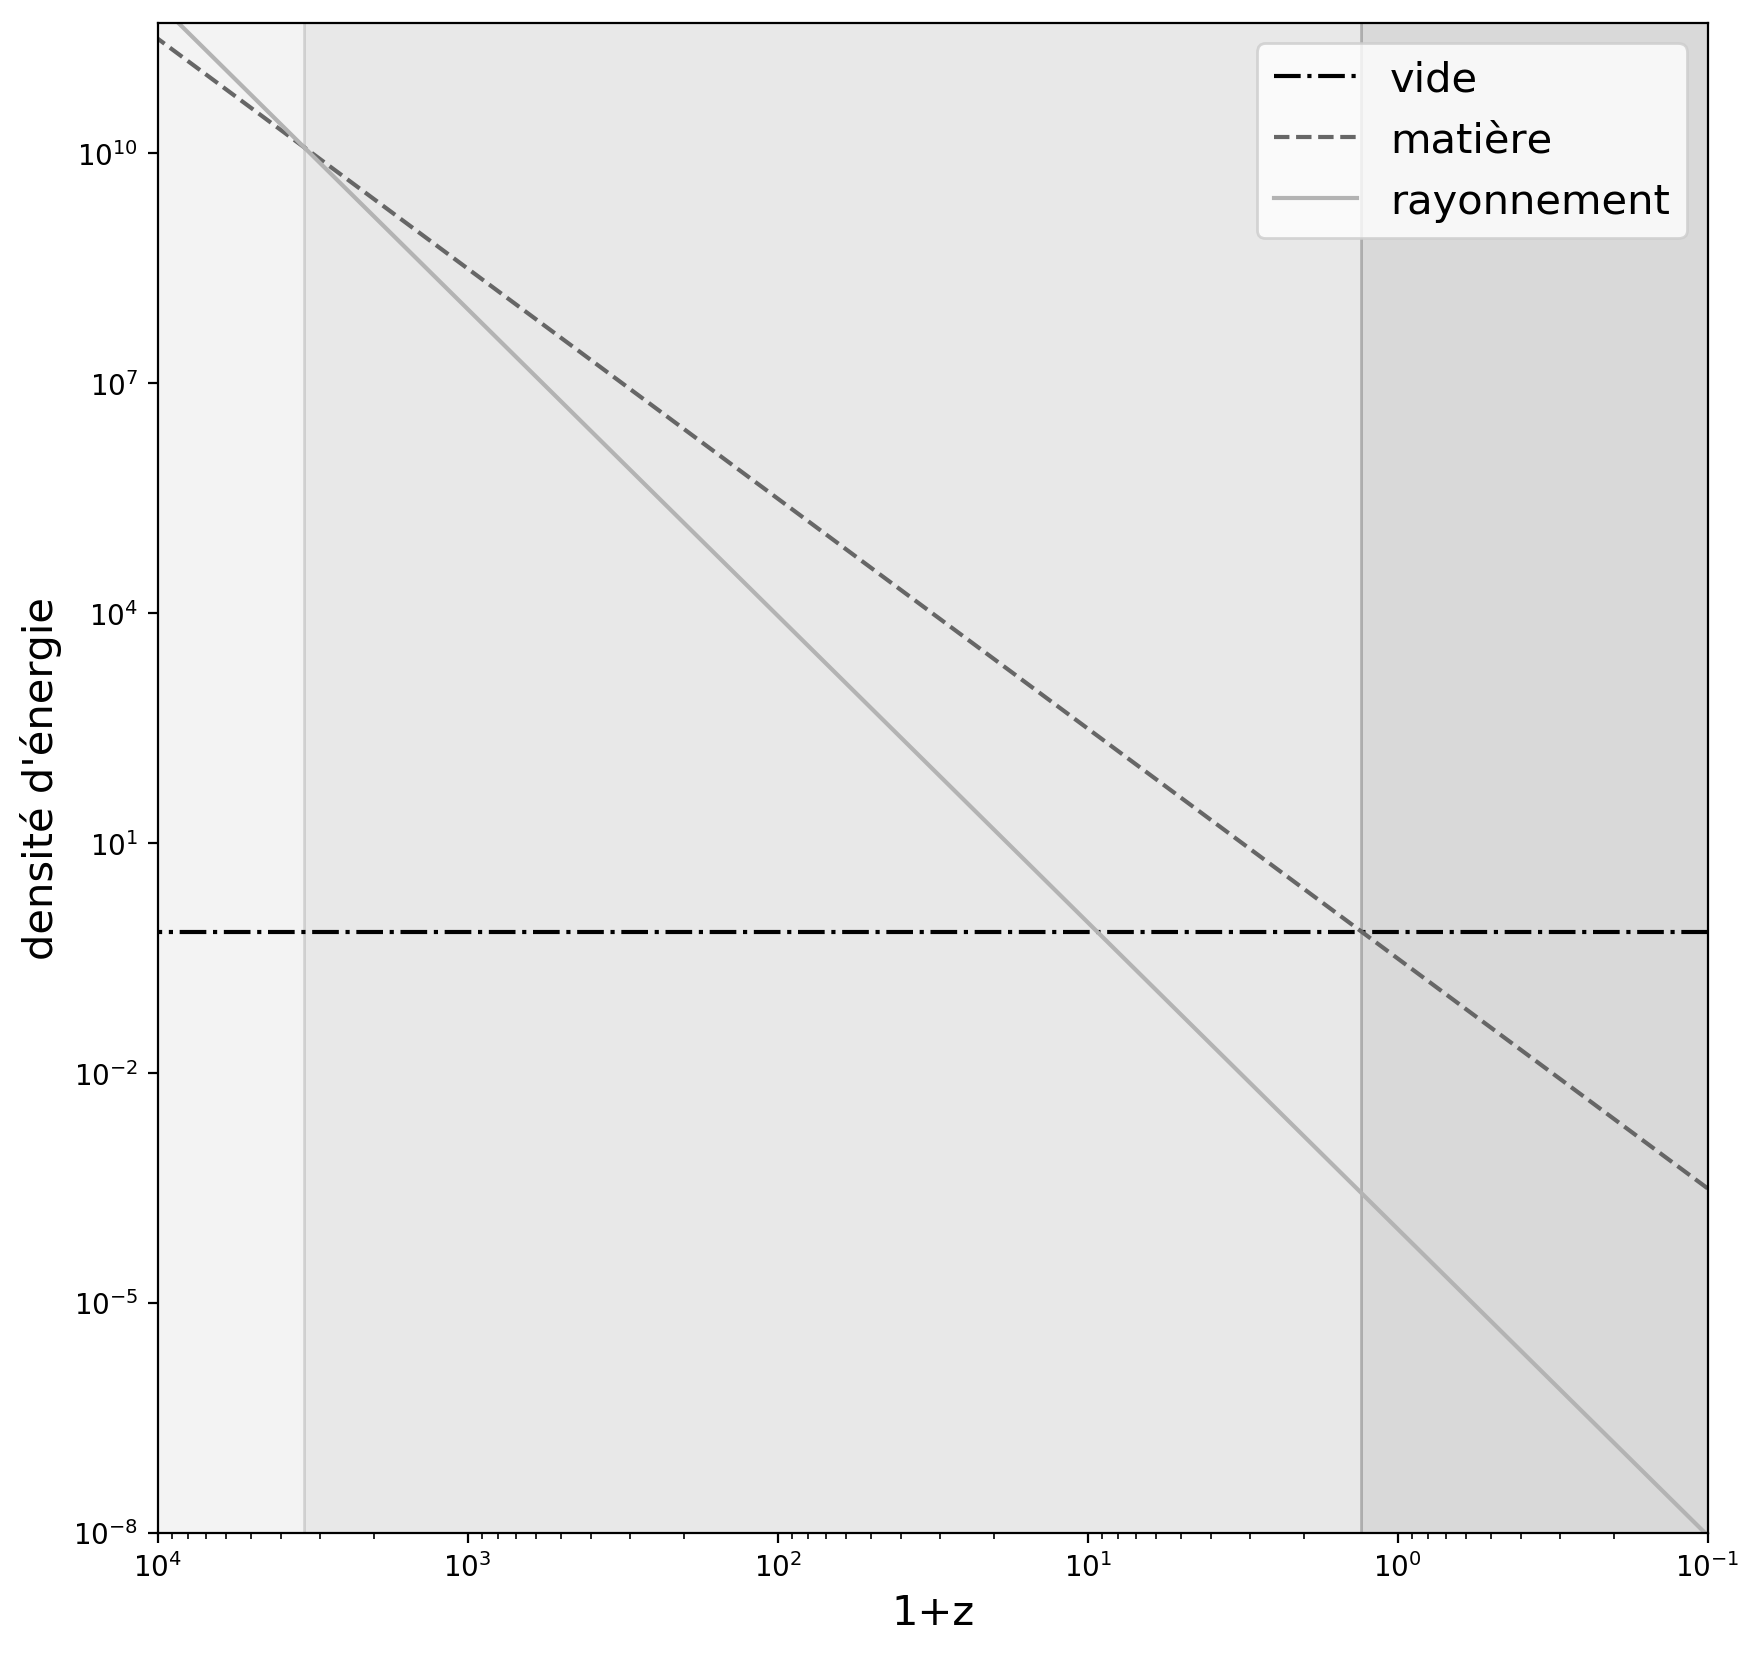
\includegraphics[height=7cm]{plots/homo/era.pdf}
	\caption{The evolution of the density of the three fluids. Radiation dominates the earliest times, followed by matter then vacuum. The parameters are $\Omega_m=0.3$, $\Omega_v=0.7$ and $h=0.7$.}
	\label{fig:plots_homo_era}
\end{figure}
The three fluids behaves differently along time. Let us assume that $a(t)$ is a growing function of time, which corresponds to what is being observed et let us consider again the variation of the 3 densities:
\begin{eqnarray}
	\rho_m&=&\rho_{m,0}a^{-3},\\
	\rho_r&=&\rho_{r,0}a^{-4},\\
	\rho_v&=&\rho_{v,0}.
\end{eqnarray}
Clearly at early times, when $a\sim 0$, the radiation will inevitably dominates. Conversely, as $a\rightarrow+\infty$, the vacuum will eventually be the dominant component. In between, the matter will compose most of the energy. These transitions are inevitable, unless one of the fluids is absent from our Universe. It means, that except during the transitions, the dynamics can be studied by assuming only one fluid, leaving the two others aside. The three eras are called \emph{radiation-}, \emph{matter-} and \emph{vacuum-dominated} era.
% subsection domination_era (end)
% section cosmological_fluids (end)

\section{Dynamics of the Universe} % (fold)
\label{sec:dynamics_of_the_universe}
Using the generalized densities $\rho+3P/c^2$ in the Friedman equation leads to:
\begin{equation}
	\frac{\ddot a}{a}=-\frac{4\pi G}{3}(\rho_m+2\rho_r-2\rho_v),
\end{equation}
which can integrated into
\begin{equation}
	H^2=H_0^2(\frac{8\pi G}{3H_0^2}\rho_T-\frac{k}{a^2H_0^2}),
	\label{eq:hubble2}
\end{equation}
$H(t)=\dot a /a$ being the usual Hubble's constant and $\rho_T$, a `total' density, being given by:
\begin{equation}
	\rho_T=\frac{\rho_{m,0}}{a^3}+\frac{\rho_{r,0}}{a^4}+\rho_{v}.
	\label{eq:rhoT}
\end{equation} 
From Eqs. \ref{eq:hubble2} and \ref{eq:rhoT}, it can easily be seen that the different components of the Universe will have a different impact on its evolution described by $a(t)$. Furthermore, the expansion factor is tightly related to the cosmic time, hence a specific composition will lead to a specific age of the Universe today. 

In order to constrain the dynamics, let us introduce the critical density (Eq. \ref{eq:rhoc}) via the density parameters:
\begin{equation}
	\Omega_{i}=\rho_{i,0}/\rho_c
\end{equation}  
into Eq. \ref{eq:hubble2}. Please note that the density parameters are related to the densities \emph{today} and could have been noted as $\Omega_{i,0}$. Usually the subscript $0$ is left aside for this quantities and $\Omega_i$ refers to the current density at $t=t_0$ in units of the critical density. Eq. \ref{eq:hubble2} becomes
\begin{equation}
	H^2=H_0^2(\frac{\Omega_m}{a^3}+\frac{\Omega_r}{a^4}+\Omega_v+\frac{\Omega_k}{a^2}),
\end{equation}
or
\begin{equation}
	{\dot a}^2=H_0^2(\frac{\Omega_m}{a}+\frac{\Omega_r}{a^2}+{\Omega_v}{a^2}+\Omega_k).
	\label{eq:adot2}
\end{equation}

We introduced a new density parameter which takes in account the integration factor $k$:
\begin{equation}
	\Omega_k=-\frac{3k}{8\pi G}.
\end{equation}
In a relativistic context it can be shown that $k$ is related to the intrinsic curvature of space. It implies that even if the three fluids of the Universe have a zero density, some curvature may still be here as a kind of initial condition. In our derivation it appears as a pure mathematical consequence of the integration of the laws of dynamics. Taking Eq. \ref{eq:adot2} at time $t=t_0$, we get:
\begin{equation}
	\Omega_k=1-(\Omega_m+\Omega_r+\Omega_v)=1-\Omega_T.
\end{equation}
Then, if the curvature $k=0$, the sum of the densities of matter, radiation and vacuum is equal to the critical density: the Universe is flat. If the Universe is heavier, $\Omega_T>1$, $\Omega_k$ is negative and its curvature $k$ is positive: the Universe has a closed geometry such as the surface of a sphere. Conversely, if the Universe is lighter than the critical value, $\Omega_T<1$ and $\Omega_k>0$ meaning that the curvature is negative, hyperbolical. We recover the conclusions of Sec. \ref{ssub:energetics}.

The evolution of the expansion factor is straightforward from Eq. \ref{eq:adot2}. We have:
\begin{equation}
	{\dot a}\equiv\frac{\md a}{\md t}=H_0\sqrt{\frac{\Omega_m}{a}+\frac{\Omega_r}{a^2}+{\Omega_v}{a^2}+\Omega_k},
\end{equation}
or
\begin{equation}
	\md t=\frac{\md a}{H_0\sqrt{{\Omega_m}{a^{-1}}+{\Omega_r}{a^{-2}}+{\Omega_v}{a^2}+\Omega_k}}.
\end{equation}
The link between time and expansion is thus established by the integral relation:
\begin{equation}
	t=H_0^{-1}\int_0^a \frac{\md a}{\sqrt{{\Omega_m}{a^{-1}}+{\Omega_r}{a^{-2}}+{\Omega_v}{a^2}+\Omega_k}},
\end{equation}
which has to be numerically integrated in the general situation.
The age of the Universe $t_0$ is easily obtained recalling $a(t_0)=1$:
\begin{equation}
	t_0=H_0^{-1}\int_0^1 \frac{\md a}{\sqrt{{\Omega_m}{a^{-1}}+{\Omega_r}{a^{-2}}+{\Omega_v}{a^2}+\Omega_k}}.
	\label{eq:univage}
\end{equation}

The age and the evolution of $a(t)$ obviously depend on the composition of the Universe. They are also related to the value of the Hubble's constant today $H_0$, stating its importance in any cosmological study. To summarize, a minimal cosmological model is defined by the amount of matter ($\Omega_m$) and radiation ($\Omega_r$), whether or not any cosmological constant (vacuum) exists ($\Omega_v$), its geometry ($\Omega_k$) and the expansion rate today ($H_0$) in order to set boundary conditions to the Friedmann equations. 
In the forthcoming sections, we will consider several models of Universe.

\subsection{Matter dominated model} % (fold)
\label{sub:einstein_de_sitter_model}
The first model is the most natural one, a flat Universe filled with matter only:
\begin{eqnarray}
	\Omega_m&=&1,\\
	\Omega_v&=&0,\\
	\Omega_r&=&0,\\
	\Omega_k&=&0.
\end{eqnarray} 
Such a model is called an \emph{Einstein-De Sitter} (EdS) Universe. Eq. \ref{eq:univage} can be modified as :
\begin{equation}
	H_0t=\int_0^a \sqrt a \md a,
\end{equation}
leading to 
\begin{equation}
	t=\frac{2}{3H_0}a^{3/2},
\end{equation}
or
\begin{equation}
	a\sim t^{2/3}.
\end{equation}
The age of the Universe is given by:
\begin{equation}
	t_0=\frac{2}{3H_0}\sim8.5\mathrm{Gyrs}
\end{equation}
the last evaluation is obtained for $H_0=75$ km/s. The evolution of this model is given if Fig. \ref{fig:plots_homo_expansion}.

This model experiences an infinite expansion which stalls at infinity: this is expected from a model with $\Omega_T=1$. A Big-Bang does happen as no singularity arise as $a\rightarrow 0$ and its initial `motion' decelerates under the influence of gravity. The expected age of the Universe is 8.5 Gyrs which is much less than the age of the stellar population of globular clusters: unless they were formed before the Big-Bang, such a model cannot explains the observations and has thus been ruled out. Still, it has been shown that the Universe is dominated by matter at intermediate times (see Sec. \ref{sub:domination_era}) and it follows the EdS evolution during this era.

% subsection einstein_de_sitter_model (end)
\subsection{Radiation dominated} % (fold)
\label{sub:radiation_dominated}
The second model is relevant for the earliest times of the Universe history. We consider a model filled by radiation exclusively:
\begin{eqnarray}
	\Omega_m&=&0,\\
	\Omega_v&=&0,\\
	\Omega_r&=&1,\\
	\Omega_k&=&0.
\end{eqnarray}
It is consistent with the radiation-dominated era just after the Big-Bang. The integration of Eq. \ref{eq:univage} is straightforward into:
\begin{equation}
	t=\frac{1}{2H_0}a^2
\end{equation}
or
\begin{equation}
	a\sim\sqrt t.
\end{equation}
% subsection radiation_dominated (end)
\subsection{Vacuum dominated} % (fold)
\label{sub:vacuum_dominated}
Logically, the third model is dominated by vacuum energy:
\begin{eqnarray}
	\Omega_m&=&0,\\
	\Omega_v&=&1,\\
	\Omega_r&=&0,\\
	\Omega_k&=&0.
\end{eqnarray}
In the sequence of domination era, this model is similar to the latter times of the Universe, where the cosmological constant dominates the cosmic energy budget. It is often called the \emph{de Sitter} model. The integral in Eq. \ref{eq:univage} becomes:
\begin{equation}
	t=H_0^{-1}\int_\epsilon^a\frac{\md a}{a},
\end{equation}
which is divergent toward zero, hence we construct the integral from a small but non-nil expansion factor $\epsilon$. This trick is does not have any consequence on further investigations since vacuum dominated era start at late times when $a$ is definitely non zero. We get:
\begin{equation}
	t=H_0^{-1}\ln \frac{a}{\epsilon},
\end{equation}
or
\begin{equation}
	a(t)=\epsilon e^{H_0 t}.
\end{equation}

The vacuum dominated model expands exponentially, thus \emph{it accelerates}, $\ddot a >0$, as predicted in Sec. \ref{sec:cosmological_fluids}. Interestingly if one calculates the Hubble's constant in this model:
\begin{equation}
	H(t)\equiv \frac{\dot a}{a}=H_0.
\end{equation}
The expansion rate is constant and $H(t)$ does not vary. Finally it should be noted that such a model does not start with a Big-Bang as $t\rightarrow-\infty$ when $\epsilon \rightarrow 0$. It can be seen on Fig. \ref{fig:plots_homo_expansion}.

This model has also an interest in the prospect of \emph{inflation}: an important growth is likely to have happen at earliest stage of the cosmic history, explaining among other things the observed homogeneity and flatness. The inflation can be modeled by a field similar to vacuum energy, leading also to an exponential expansion. 
% subsection vacuum_dominated (end)

\begin{figure}[htbp]
	\centering
		\includegraphics[height=7cm]{plots/homo/expansion.pdf}
	\caption{The expansion factor as a function of time. Lookback time is equal to zero today. The LCDM model corresponds to the concordance cosmology $\Omega_m=0.24$ and $\Omega_v=0.76$.}
	\label{fig:plots_homo_expansion}
\end{figure}% section dynamics_of_the_universe (end)

\section{The Friedmann-Robertson-Walker metric} % (fold)
\label{sec:the_friedmann_robertson_walker_metric}
From now on, we will drop the simple newtonian description in order to deal with the general relativity description of cosmology. The focus will be put on a simple description of the formalism and the student would surely benefit to refer to specialized books for a more complete treatment.

\subsection{metrics \& geometry} % (fold)
\label{sub:metrics_&_geometry}
A \emph{metric} allows to compute the distance between two points, even though the geometry of the considered space can be quite complex.

In the regular euclidian space, the square of the distance between two points $\md s^2$ is given by:
\begin{equation}
	\md s^2=\md x^2+\md y^2+\md z^2.
\end{equation}
This distance can be expressed by means of a metric $E_{\mu\nu}$ giving
\begin{equation}
	\md s^2=\sum_{\mu=1}^{3}\sum_{\nu=1}^{3}E_{\mu\nu}\md x^\mu\md x^\nu\equiv E_{\mu\nu}\md x^\mu\md x^\nu,
\end{equation}
where the last relation uses the Einstein's notation where summation is performed over repeated indices. The euclidian metric is given by
\begin{eqnarray}
	E_{\mu\nu}&=1&\mu=\nu,\\
	E_{\mu\nu}&=0&\mu\ne\nu.
\end{eqnarray}

In a flat space-time points are called \emph{events} and are defined by $x^\mu$, the distance between two \emph{events} is given by
\begin{equation}
	\md s^2=-\eta_{\mu\nu}\md x^\mu \md x^\nu=c^2\md t^2 -(\md x^2+\md y^2+\md z^2),
\end{equation}
where the \emph{Minkowski} metric is defined by:
\begin{eqnarray}
	\eta_{00}&=-1&,\\
	\eta_{\alpha\beta}&=1&\alpha=\beta\\
	\eta_{\mu\nu}&=0&\mu\ne\nu.
\end{eqnarray}
Other conventions exists (e.g. with a (+,-,-,-) trace for the metric), we will use the one defined in \emph{Gravitation \& Cosmology}. 

The quantity $\md s^2$ is called \emph{the adiabatic invariant} and is constant as one switch from one inertial frame to another. Clearly $\md s^2$ can be negative, but events separated by such a distance cannot be associated to a physical propagation since it implies (dropping the two other dimensions) $\md x/\md t >c$. If we consider a particle traveling a distance $\md x$ during $\md t$, the adiabatic invariant is related to the \emph{proper time}, i.e. the amount of time spent between the two events by an observer attached to the particle:
\begin{equation}
c\md \tau=\md s.	
\end{equation}
Massless particles (such as photons) follow trajectories that satisfy $\md s=0$ and their velocity is therefore equal to $c$ in every inertial frame.

For an homogeneous and isotropic Universe, the geometry is defined by the Robertson-Walker metric where the relativistic invariant becomes~:
\begin{equation}
\md s^2=c^2\md t^2-a(t)^2(\frac{\md r_0^2}{1-Kr_0^2}+r_0^2\md\theta^2+r_0^2\sin^2\theta\md\phi^2),
\label{eq:FRW}
\end{equation}
given here in spherical comoving coordinates. 
A quick inpection of Eq. \ref{eq:FRW} shows that $K$ has the dimension of the inverse square of a length:
\begin{equation}
	K=\pm\frac{1}{R^2}.
\end{equation}
The $R$ quantity identifies itself with the \emph{curvature radius} of the Universe. A flat Universe implies $R\rightarrow \infty$ thus $K=0$. An open universe has $K<0$ while a closed Universe has $K>0$.

\begin{figure}[htbp]
	\centering
		\includegraphics[height=5cm]{plots/homo/hyper3D2.png}
		\includegraphics[height=5cm]{plots/homo/sphere3D2.png}
	\caption{Circles (in red) in non-euclidian geometries: hyperbolical (left) and spherical (right).}
	\label{fig:plots_homo_hyper3D2}
\end{figure}
As already stated, an open model corresponds to an hyperboloidal geometry while a closed one corresponds to spherical geometry. It can be shown by considering the ratio of a circle circumference $C$ to its radius $r$. As shown by Fig. \ref{fig:plots_homo_hyper3D2}, it depends on the underlying space geometry. For a flat space this ratio is obviously:
\begin{equation}
	\frac{C}{r}=\frac{2\pi r}{r}=2\pi.
\end{equation}
\begin{figure}[htbp]
	\centering
		\includegraphics[height=5cm]{plots/homo/spherical.pdf}
	\caption{Notation for a circle in spherical geometry.}
	\label{fig:plots_homo_spherical}
\end{figure}
On a sphere the situation is slightly different (see Fig. \ref{fig:plots_homo_spherical}). The circumference is given by the usual formulae $2\pi\rho$, but the radius measured by an observer on the surface is given by $r=R\Psi=R\arcsin(\rho/R)$. Hence, the previous ratio is modified as :
\begin{equation}
	\frac{C}{r}=\frac{2\pi \rho}{R\arcsin(\rho/R)}<2\pi
	\label{eq:ratio}
\end{equation}

How does it relate to the RW metric ? Taking only the spatial part of the metric and assuming that the origin lies at the circle center, the radius $r$ is obtained assuming a fixed direction $(\theta,\phi)$:
\begin{equation}
	r=a(t)\int\frac{\md r_0}{\sqrt{1-Kr_0^2}}=a(t)R\arcsin{(r_0/R)},
\end{equation}
while the circumference is given by $C=2\pi a(t)r_0$. The ratio of the primer to the latter is identical to the relation \ref{eq:ratio} and $K$ appears naturally as the inverse square of the `sphere' radius $R$.

The hyperbolic case is less intuitive. Following the same procedure as in the spherical case the radius is given by:
\begin{equation}
		r=a(t)\int\frac{\md r_0}{\sqrt{1+(r_0/R)^2}}=a(t)R\sinh^{-1}(r_0/R),
\end{equation}
where $K=-1/R^2$, consistent with a open geometry. Consequently, the circumference to radius ratio is given by:
\begin{equation}
	\frac{C}{r}=\frac{2\pi a(t) r_0}{a(t)R\sinh^{-1}(r_0/R)}>2\pi.
\end{equation}

These circle experiments are purely illustrative. Of course, the observers are never in a position to draw a circle around themselves to test the geometry of the Universe. Instead they test the angles of remarkable triangles as introduced in section \ref{ssub:energetics} and Fig. \ref{fig:plots_homo_990006b}. It will be discussed in more details in Ch. \ref{cha:the_cosmic_microwave_background}.
% subsection metrics_&_geometry (end)
\subsection{Redshift and expansion} % (fold)
\label{sub:redshift_and_expansion}
Having access to the generic form of the metric let us consider two points A and B and A emits a first light signal toward B at time $t_A$ and a second one $t_A+\delta t_A$ shortly after. The first signal is received by B at time $t_B$ and the second is received at time $t_B+\delta t_B$. Our common sense dictates that $\delta t_A=\delta t_B$, but the interplay of propagation and expansion will break this intuition.

Since we consider light signals, the events `emitted in A' and `received in B' are separated by a zero interval. Plus if we consider a pure radial motion, we get an infinitesimal interval:
\begin{equation}
	0=c^2\md t^2-a(t)^2\frac{\md r_0^2}{1-Kr_0^2},
\end{equation}
hence along the trajectory from A to B:
\begin{equation}
	c\int_{t_A}^{t_B}\frac{\md t}{a}=\int_A^B\frac{\md r}{\sqrt{1-Kr}}.
\end{equation}
Of course the same relation holds for the second signal:
\begin{equation}
	c\int_{t_A+\delta t_A}^{t_B+\delta t_B}\frac{\md t}{a}=\int_A^B\frac{\md r}{\sqrt{1-Kr}}.
\end{equation}
Since the r.h.s of these relations does not depend on the instant of the emission, the relation:
\begin{equation}
	c\int_{t_A+\delta t_A}^{t_B+\delta t_B}\frac{\md t}{a}=c\int_{t_A}^{t_B}\frac{\md t}{a},
\end{equation}
holds for every pair of instants $t_A$ and $t_B$. It leads to 
\begin{equation}
	\int_{t_A}^{t_A+\delta t_A}\frac{\md t}{a}=\int_{t_B}^{t_B+\delta t_B}\frac{\md t}{a}
	\end{equation}
and
\begin{equation}
	\frac{\delta t_A}{a(t_A)}=\frac{\delta t_B}{a(t_B)}.
	\label{eq:dilatation}
\end{equation}

Let $\delta t_A$ be the period of an electromagnetic wave and its wavelength is given by $\lambda_A=c\delta t_A$. Eq. \ref{eq:dilatation} states that the wavelength of the radiation is modified as it travels from A to B:
\begin{equation}
	\frac{\lambda_A}{a(t_A)}=\frac{\lambda_B}{a(t_B)},
\end{equation}
or
\begin{equation}
	\frac{\lambda_B-\lambda_A}{\lambda_A}=\frac{a(t_B)}{a(t_A)}-1
\end{equation}

Assuming that the signal is received today when $a_B=1$, the usual definition for the redshift $z=1/a-1$ is recovered. Interestingly, this relation states that the redshift is not related to any kind of motion, as an interpretation based on Doppler effect would naturally emphasize. Conversely, the redshift is really a measure of the ratio of the expansion factors of emission and reception, it directly measures an element of the Universe's metric. 

It should also be noted that Eq. \ref{eq:dilatation} holds for any pair of events distant by a certain duration $\delta t_A$ and therefore states that one should expect a generic dilation of any temporal evolution when we measure them at cosmological distances: any rate must decrease in an expanding Universe. There are models which explains redshift by `tired light', where photons loose their energy as they travel, and avoid any kind of expansion. Such models don't predict such a dilatation of time intervals and if rates are effectively seen as decreasing, it would rule them out.
% subsection redshift_and_expansion (end)
\subsection{Distances in cosmology} % (fold)
\label{sub:distances_in_cosmology}
Measuring distances is definitely difficult in cosmological sciences but \emph{defining} them is also a real challenge.

\paragraph{Comoving Distance} % (fold)
\label{par:comoving_distance}
The \emph{comoving distance} $r_0$ has already been introduced and does not change with expansion. More generally we can define a set of comoving coordinates by noting that freely falling particles must obey the relation:
\begin{equation}
	\frac{\md^2 x^\mu}{\md t^2}+\Gamma^\mu_{\nu\lambda}\frac{\md x^\nu}{\md t}\frac{\md x^\lambda}{\md t}=0,
\end{equation}
which is the covariant version of the second time derivative of the position. $\Gamma^\mu_{\nu\lambda}$ is the usual affine connection given by:
\begin{equation}
	\Gamma^\mu_{\nu\lambda}=\frac{1}{2}g^{\mu\kappa}\left[\frac{\partial g_{\kappa\nu}}{\partial x^\lambda}+\frac{\partial g_{\kappa\lambda}}{\partial x^\nu}-\frac{\partial g_{\nu\lambda}}{\partial x^\kappa}\right].
\end{equation}
From Eq. \ref{eq:FRW}, one can note that $\Gamma^i_{00}=0$, hence:
\begin{equation}
	\frac{\md^2 x^i}{\md t^2}=0.
\end{equation}
Particles at rest in these coordinates $(r_0,\theta,\phi)$ will remain at rest even though the Universe physically expands (or shrink): this defines real comoving coordinates and distances. The proper time is directly given by $t$, measured by comoving clocks.

One can ask what is the comoving distance of an object seen today with a redshift $z=1/a-1$ ? Again, the RW metric will provide the answer. Assuming that photons are casted along a direction $(\theta,\phi)=(0,0)$, the relativistic invariant is:
\begin{equation}
	\md s^2=c^2\md t^2-a(t)^2\frac{\md r_0^2}{1-Kr_0^2}=0,
\end{equation} 
the last equality coming from the fact that photons are massless and therefore follow path such as $\md s=0$. Consequently for a photon produced at $t_e$ and received by the observer today at $t_0$, we have:
\begin{equation}
	c\int_{t_e}^{t_0}\frac{\md t}{a(t)}=\int_0^{r_0} \frac{\md r}{\sqrt{1-Kr^2}}=S_K(r_0),
\end{equation}
where $S_K(r_0)$ is defined as 
\begin{equation}
	S_K(r_0)=
	\begin{cases}
	\frac{1}{\sqrt {|K|}}	\sin^{-1}{r_0\sqrt K}, &\text{ if } K>0\\
	r_0, &\text{ if } K=0\\
	\frac{1}{\sqrt {|K|}}	\sinh^{-1}{r_0\sqrt |K| }, &\text{ if } K<0
	\end{cases}
\end{equation}
and assuming a cosmological model to compute $a(t)$, it is possible to recover the comoving distance from $z$. If we define $\chi$ as
\begin{equation}
	\chi=c\int_{t_e}^{t_0}\frac{\md t}{a(t)}=c\int_{a_e}^{a_0}\frac{\md a}{H(a)a^2}=c\int_{z_0}^{z_e}\frac{\md z}{H(z)},
\end{equation}
an object with a redshift $z$ has a comoving distance given by
\begin{equation}
	r_0(z)=
	\begin{cases}
		\frac{1}{\sqrt{|K|}}\sin{\sqrt{|K|}\chi}, &\text{ if } K>0\\
		\chi, &\text{ if } K=0\\
		\frac{1}{\sqrt{|K|}}\sinh{\sqrt{|K|}\chi}, &\text{ if } K<0.
	\end{cases}
	\label{eq:comovz}
\end{equation}
% paragraph comoving_distance (end)

\paragraph{Proper Distance} % (fold)
\label{par:proper_distance}
The \emph{physical distance} or \emph{proper distance} $r$ is measured at time $t$ from the origin to an object at comoving distance $r_0$:
\begin{equation}
	r=a(t)\int_0^{r_0}\frac{\md r_0}{\sqrt{1-Kr_0^2}}=aS_K(r_0)
\end{equation}
which gives the usual $r=a r_0$ in the case of flat geometry. Since the integral is constant with time for a given pair of objects, the rate of change of the proper distance is given by:
\begin{equation}
	\dot r=\frac{\dot a}{a}r=H(t)r.
\end{equation}

Several points should be mentioned at this stage. The first important point is that the Hubble law involves the proper distance. The second important thing in this relation is the fact that it is established for a pair of objects (including the observer at the origin) \emph{at the same proper time t}. The third important fact is that \emph{velocities $\dot r$ can be greater than c !} This last point is investigated in further details in the following section.
% paragraph proper_distance (end)

\paragraph{Luminous Distance} % (fold)
\label{par:luminous_distance}
In principle, luminous fluxes can help us to determine a distance to an object. Let $L$ be its intrinsic luminosity (energy per unit time) and $d$ its distance, the observed flux $F$ (energy per unit time and unit area) is given by the well-known relation:
\begin{equation}
	F=\frac{L}{4\pi d^2},
\end{equation}
the energy is spread over the surface of a sphere centered on the source. 

When cosmological expansion is taken in account, several additional effects should be considered:
\begin{itemize}
	\item the energy is spread over a sphere of constant $r_0$. According to the metric and integrating over all the angles $(\theta,\phi)$, its \emph{proper} area is given by $4\pi a(t_0)^2r_0^2$.
	\item $L$ is a rate, therefore it is the subject of the time dilatation described in sec. \ref{sub:redshift_and_expansion}. If we assume that the source emits N photons during $\delta t_e$, these same photons are received at a rate:
	\begin{equation}
		\dot N(t_0)=\frac{N}{\delta t_0}=\frac{N}{\delta t_e a(t_0)/a(t_e)}=\frac{\dot N(t_e)}{1+z}
	\end{equation}
	according to Eq. \ref{eq:dilatation}. Thus the luminosity should be decreased by a factor $1+z$.
	\item Each photon is emitted with an energy $h\nu_e$ and received with an energy $h\nu_0=h\nu_e/(1+z)$. Thus the luminosity should be decreased by an additional $1+z$ factor.
\end{itemize}

Consequently, the observed flux is given by:
\begin{equation}
	F=\frac{L}{4\pi a^2(t_0)r_0^2(1+z)^2}
\end{equation} 
and by analogy with the conventional definition of $F$ we can define a \emph{luminous distance} by:
\begin{equation}
	d_L=r_0(z) (1+z),
	\label{eq:lumdist}
\end{equation}
where we applied the usual convention $a(t_0)=1$.
When one measure a distance from the luminosity of distant objects like supernovae or galaxies, the distance measured is $d_L$.
% paragraph luminous_distance (end)
\paragraph{Angular distance} % (fold)
\label{par:angular_distance}
An additional way to compute a distance uses angles on the sky. In Euclidian geometry, if an object of transversal extent $s$ is seen with an angle $\theta$, we have:
\begin{equation}
	s=d_A\theta,
\end{equation} 
where $d_A$ is the \emph{angular diameter distance}.

In a cosmological context, this distance is affected by expansion. First let us note that the (small) proper size of the object at the instant of emission $t_e$ is given by:
\begin{equation}
	\delta s=a(t_e)r_0\delta\theta.
\end{equation}
Then let us recall that $a(t_e)=(1+z)^{-1}$. By analogy with the Euclidian expression we simply get
\begin{equation}
	d_A=a(t_e)r_0=\frac{r_0(z)}{1+z}.
\end{equation}
By comparison with Eq. \ref{eq:lumdist} we get the relation between the angular diameter distance and the luminous distance:
\begin{equation}
	d_A=\frac{d_L}{(1+z)^2}.
\end{equation}

Clearly if one can measure $d_A$, $d_L$ won't bring more information and vice-versa. However, it is difficult to measure $d_A$ for point-like or fuzzy objects and the focus will be put on $d_L$. Conversely, $d_A$ is central in the study of gravitational lenses and the structures of CMB anisotropies.
% paragraph angular_distance (end)
\begin{figure}[htbp]
	\centering
		\includegraphics[height=16cm]{plots/homo/dist.pdf}
	\caption{The distances for an object seen with a redshift $z$ in units of the Hubble radius. Solid curves stand for Einstein-De Sitter calculations, while dashed ones correspond to the concordance model LCDM ($\Omega_m=0.27, \Omega_v=0.73$).}
	\label{fig:plots_homo_dist}
\end{figure}

% subsection distances_in_cosmology (end)
% section the_friedmann_robertson_walker_metric (end)

% chapter the_homogeneous_universe (end)
